\section{K-means Clustering}

\begin{figure}[h!]
\centering
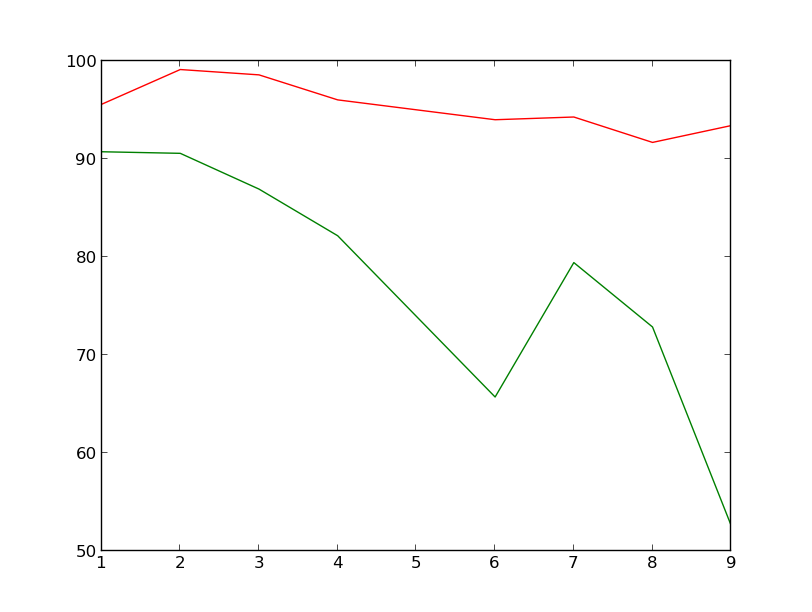
\includegraphics[width=0.8\textwidth]{images/kmeans_2_centers.png}
\caption{A plot of the centroids of the clusters discovered through k-means clustering with 2 clusters. x-axis is the features, y-axis is score (\%)}
\label{fig:kmeans_2_centers}
\end{figure}

\begin{figure}[h!]
\centering
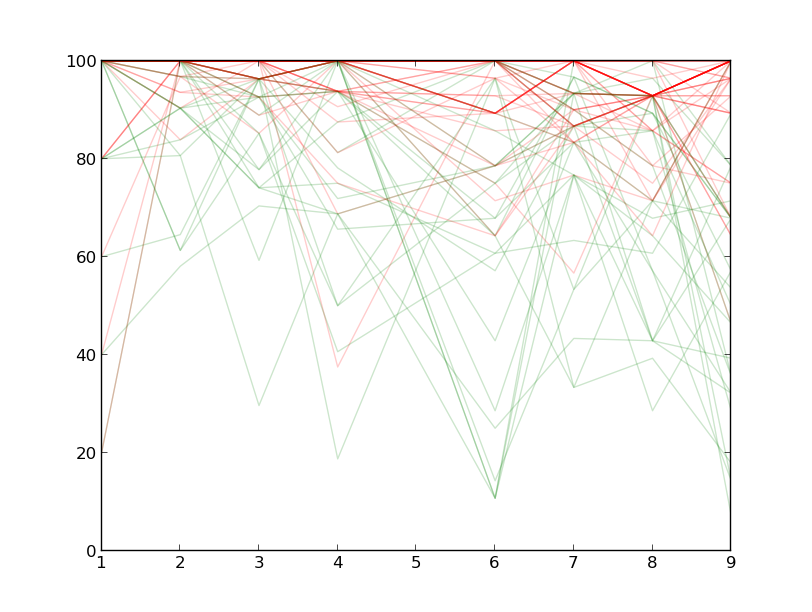
\includegraphics[width=0.8\textwidth]{images/kmeans_2.png}
\caption{A plot of all the students that submitted for each exercise. They are plotted with an opacity of 0.2 and the colours represent the cluster which they belong to after performing k-means cluster with 2 clusters. x-axis is the features, y-axis is score (\%)}
\label{fig:kmeans_2}
\end{figure}

\begin{figure}[h!]
\centering
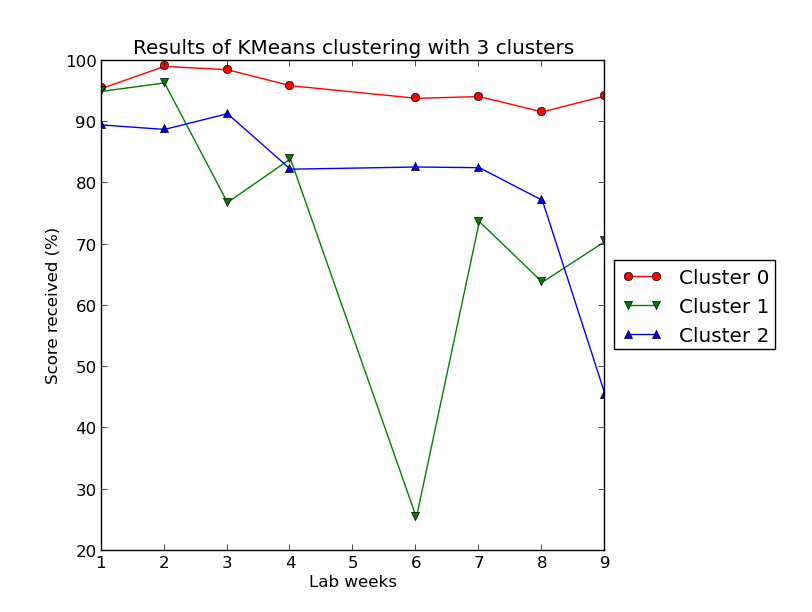
\includegraphics[width=0.8\textwidth]{images/kmeans_3_centers.png}
\caption{A plot of the centroids of the clusters discovered through k-means clustering with 3 clusters. x-axis is the features, y-axis is score (\%)}
\label{fig:kmeans_3_centers}
\end{figure}

\begin{figure}[h!]
\centering
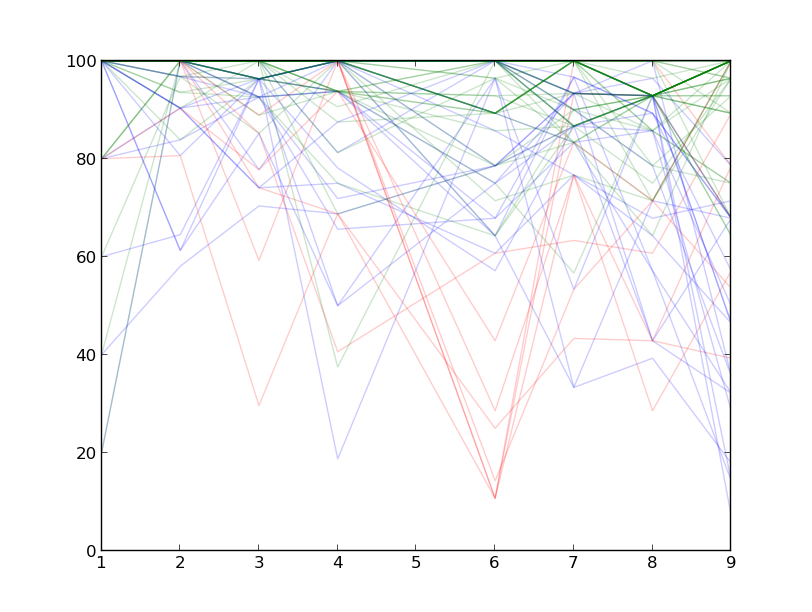
\includegraphics[width=0.8\textwidth]{images/kmeans_3.png}
\caption{A plot of all the students that submitted for each exercise. They are plotted with an opacity of 0.2 and the colours represent the cluster which they belong to after performing k-means cluster with 3 clusters. x-axis is the features, y-axis is score (\%)}
\label{fig:kmeans_3}
\end{figure}

\begin{figure}[h!]
\centering
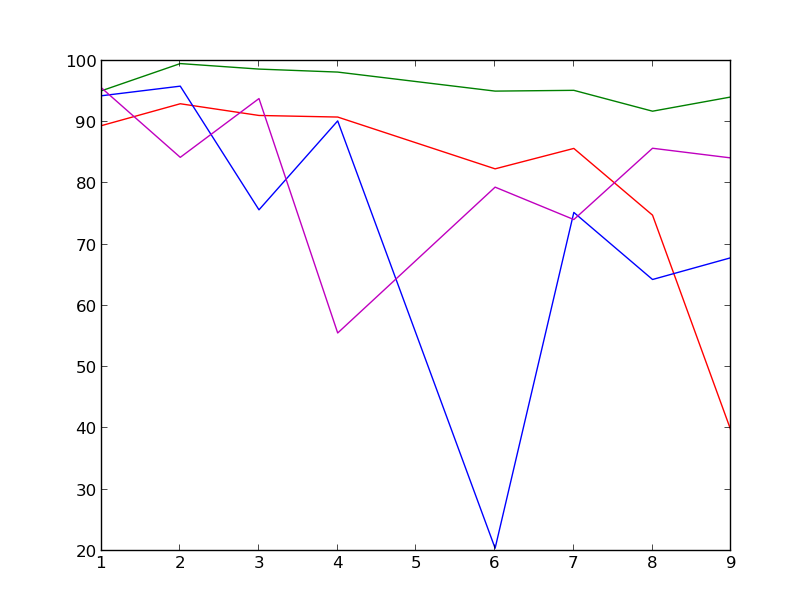
\includegraphics[width=0.8\textwidth]{images/kmeans_4_centers.png}
\caption{A plot of the centroids of the clusters discovered through k-means clustering with 4 clusters. x-axis is the features, y-axis is score (\%)}
\label{fig:kmeans_4_centers}
\end{figure}

\begin{figure}[h!]
\centering
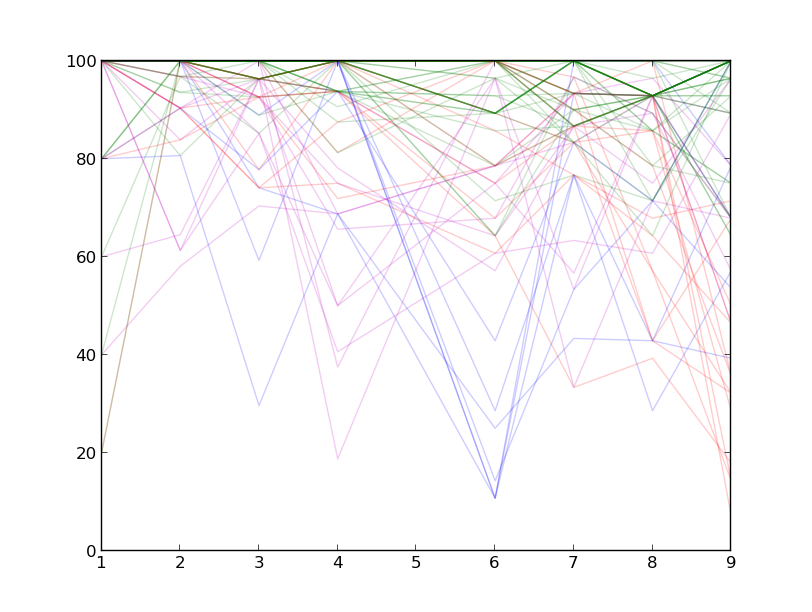
\includegraphics[width=0.8\textwidth]{images/kmeans_4.png}
\caption{A plot of all the students that submitted for each exercise. They are plotted with an opacity of 0.2 and the colours represent the cluster which they belong to after performing k-means cluster with 4 clusters. x-axis is the features, y-axis is score (\%)}
\label{fig:kmeans_4}
\end{figure}
